\part{Architecture}

\section{Decoder-Only Fundamentals \label{sec_decoder_only} }

The Transformers architecture \cite{vaswani2017attention}, which dominates Natural Language
Processing (NLP) as of July 2023, is a relatively simple architecture. There are various flavors and
variants of Tranformers, but focus here on the decoder-only versions which underlie the
GPT models \cite{gpt2radford2019language, gpt3brown2020language, gpt4openai2023}.

The full decoder-only architecture can be seen in Fig.~\ref{fig_transformers_architecture}. The
parameters which define the network can be found in App.~\ref{app_conventions}.
\begin{figure}[ht]
	\centering
	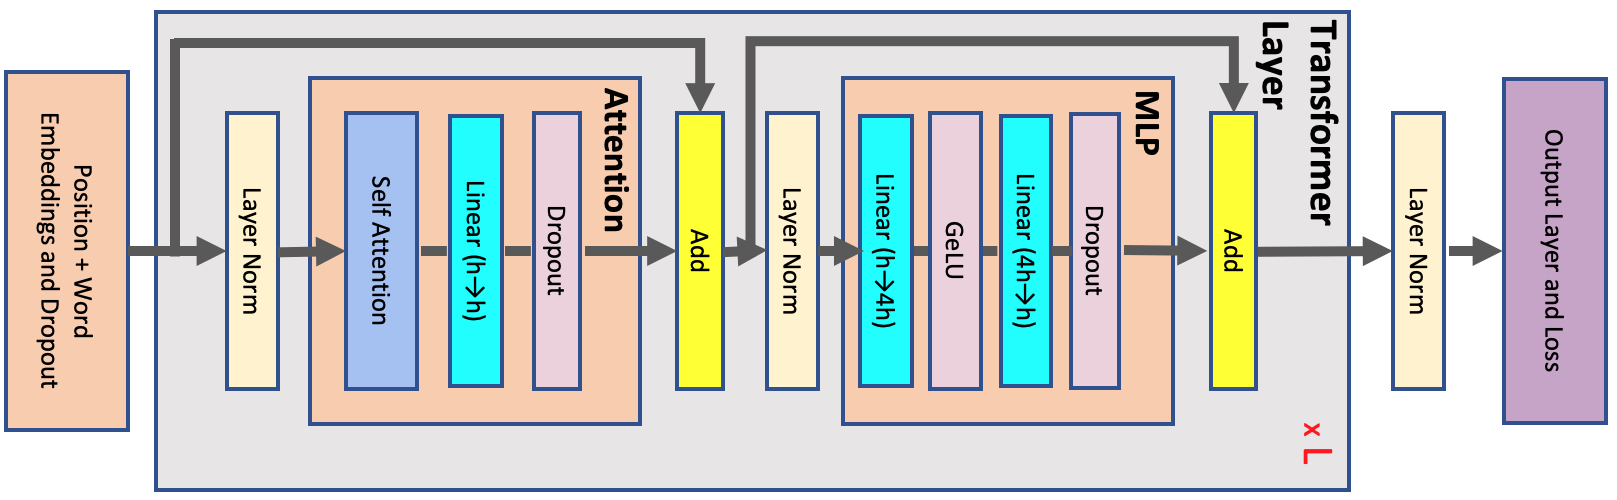
\includegraphics[scale=0.28]{figures/transformer-general.jpg}
	\caption{The full transformers architecture. Diagram taken from \cite{korthikanti2022reducing} }
	\label{fig_transformers_architecture}
\end{figure}

At a high level, decoder-only transformers take in an ordered series of word-like objects, called
tokens, and are trained to predict the next token in the sequence. Given some initial
text, transformers can be used to give a prediction for the likelihood of any possible continuation
of that text. An outline of the mechanics\footnote{This describes the vanilla architecture; almost
every component is modified in the available variants.}:
\begin{enumerate}
	\item Raw text is \textbf{tokenized} and turned into a series of integers\footnote{There are
		      about \href{https://github.com/ray-project/llm-numbers}{1.3 tokens per word}, on average.} whose values lie in \pyinline{range(V)}, with $ V $ the vocabulary
	      size.
	\item The tokenized text is chunked and turned into \pyinline{(B, S)}-shaped (batch size and
	      sequence length, respectively) integer tensors, $ x _{ bs } $.
	\item The \textbf{embedding layer} converts the integer tensors into continuous representations of shape
	      \pyinline{(B, S, D)}, $ z _{ bsd } $, with $ D $ the size of the hidden dimension.
	      \textbf{Positional encodings} have also been added to the tensor at this stage to help the
	      architecture understand the relative ordering of the text.
	\item The $ z _{ bsd } $ tensors pass through a series of transformer blocks, each of which has
	      two primary components:
	      \begin{enumerate}
		      \item In the \textbf{attention} sub-block, components of $ z _{ bsd } $ at different
		            positions ($ s $-values) interact with each other, resulting in another \pyinline{(B, S, D)}-shaped
		            tensor, $  z' _{ bsd } $.
		      \item In the \textbf{MLP} block, each position in  $ z' _{ bsd } $ is processed
		            independently and in parallel by a two-layer feed-forward network, resulting once more
		            in a \pyinline{(B, S, D)}-shaped tensor.
	      \end{enumerate}
	      Importantly, there are \textbf{residual connections} around each of these\footnote{This
		      gives rise to the concept of the \textbf{residual stream} which each transformer block reads
              from and writes back to repeatedly.} (the arrows in
              Fig.~\ref{fig_transformers_architecture}), meaning that the output of each block is
              added back to its original input.
	\item Finally, we convert the \pyinline{(B, S, D)}-shaped
	      tensors to \pyinline{(B, S, V)}-shaped ones, $ y _{ bsv } $. This is the role of
	      the \textbf{language model head} (which is often just the embedding layer used in an inverse
	      manner.)
	\item  The $ y _{ bsv } $ predict what the next token will be, i.e. $ x _{ bs+1 } $, having seen the \textbf{context}
          of the first $ s $ tokens in the sequence. Specifically, removing the batch index for
          simplicity, a \pyinline{Softmax}  of $ y _{ sv } $ gives the conditional probability $ p _{ sv
          } = P(t _{ s+1 }|t _{ s } \ldots t _ {0}) $ for the indicated series of tokens. Because of
          the chain rule of probability, these individual probabilities can be combined to form the
          probability that any sequence of tokens follows a given initial seed\footnote{In more
          detail, these probabilities are created by products: $ P(t _{ s+n } \ldots t _{ s+1}| t _{
          s } \ldots  t _{ 0 }) =P(t _{ s+n }| t _{ s+n - 1} \ldots  t _{ s } \ldots  t _{ 0}) \times
      \ldots  \times P(t _{ s+1 } | t _{ s } \ldots  t _{ 0 }) $.}.
\end{enumerate}


Each batch (the $ b $-index) is processed independently. We omitted \pyinline{LayerNorm} and
\pyinline{Dropout} layers above, as well as the causal mask; these will be covered below as we step
through the architecture in more detail.



\subsection{Embedding Layer and Positional Encodings \label{subsubsec_embedding_and_pe} }

The \textbf{embedding} layer is just a simple look up table: each of the \pyinline{range(V)} indices
in the vocabulary is mapped to a $ D $-dimensional vector via a large \pyinline{(V, D)}-shaped
table/matrix. This layer maps $ x _{ bs } \longrightarrow z _{ bsd } $. In \pyinline{torch}, this is
an \pyinline{nn.Embedding(V, D)} instance.

To each item in a batch, we add identical \textbf{positional encodings} to the vectors above with
the goal of adding fixed, position-dependent correlations in the sequence dimension which will
hopefully make it easier for the architecture to pick up on the relative positions of the inputs
\footnote{Positional encodings and the causal mask are the only components in the vanilla transformers
	architecture which carry weights with a dimension of size $ S $; i.e. they are the only parts that
	have explicit sequence-length dependence. A related though experiment: you can convince yourself
	that if the inputs $ z_{ bsd } $
	were just random noise, the transformers architecture would not be able to predict
	the $ s $-index of each such input in the absence of positional encodings. } This layer maps $ z _{
			bsd} \leftarrow z _{ bsd } + p _{ sd } $, with $ p _{ sd } $ the positional encoding tensor.

The above components require $ (V+S)D \approx VD $ parameters per model.



\subsection{Layer Norm \label{subsubsec_layer_norm} }

The original transformers paper \cite{vaswani2017attention} put \pyinline{LayerNorm} instances after
the \textbf{attention} and \textbf{MLP} blocks, but now it is common \cite{xiong2020layer} to put
them before these blocks\footnote{Which makes intuitive sense for the purposes of stabilizing the
	matrix multiplications in the blocks}.

The \pyinline{LayerNorm} operations acts over the hidden dimension (since this is the dimension the
subsequent \pyinline{Linear} instances act on). Spelling it out, given the input tensor $ z _{ bsd }
$ whose mean and variance over the $ d $-index are $ \mu _{ bs } $ and $ \sigma _{ bs } $,
respectively, the \pyinline{LayerNorm} output is
\begin{align}
	z _{ bsd } & \leftarrow \left ( \frac{ z _{ bsd } - \mu _{ bs } }{ \sigma _{ bs } } \right )\times \gamma _{ d }
	+ \beta _{ d } \equiv \LN_{ d }\, z _{ bsd}
\end{align}
where $ \gamma _{ d }, \beta  _{ d } $ are the trainable scale and bias parameters. In
\pyinline{torch}, this is a \pyinline{nn.LayerNorm(D)} instance.
Since there are two \pyinline{LayerNorm} instances in each transformer block, these components require
$ 2D $ parameters per layer.

We will continue discussing \pyinline{LayerNorm} instances in what follows in order to adhere to the
usual construction and to discuss methods like sequence-parallelism in their original form (see
Sec.~\ref{subsec_seq_parallelism}), but note: the data-independent \pyinline{LayerNorm}
transformations due to $  \gamma _{ d }, \beta _{ d } $ are completely redundant when immediately
followed by a \pyinline{Linear} layer, since both act linearly on their inputs and \pyinline{Linear}
is already the most general data-independent linear transformation. Explicitly, the  $ \gamma _{ d
}, \beta _{ d } $ parameters can be absorbed into the \pyinline{Linear} parameters:
\begin{align}
	\left (     x _{ bsd } \gamma _{ d } + \beta _{ d } \right )  W _{d d'}    + b _{ d' } & = x _{ bsd }
	W' _{ d d' } + b' _{ d' } \ , \quad W' _{ d d' } \equiv  \gamma _{  d} W _{ d d' } \ , \quad b' _{
	d' } \equiv b _{ d' } + \beta _{ d }W _{ d d' } \ ,
\end{align}
for arbitrary $ x _{ bsd } $. That is, these transformations can be equivalently performed by the
weight matrix and bias (if included) in \pyinline{Linear} layer\footnote{Note the importance of
    data-independence here: the data-dependent mean and standard deviation terms cannot be similarly
    absorbed.  Also, because the usual training algorithms are not invariant under parameter
    redefinitions, the above unfortunately does not imply that removing the learnable
    \pyinline{LayerNorm} parameters (\pyinline{elementwise_affine=False} in \pyinline{torch}) will
have no effect on training dynamics. $ \gamma _{ d }, \beta _{ d } $ can shoved into the
\pyinline{Linear} layer's parameters as a small inference-time optimization, though.}.

\subsection{Causal Attention \label{subsubsec_attn_layer} }

\textbf{Causal attention} is the most complex layer. It features $ A $  sets of weight
matrices\footnote{There are also bias terms, but we will often neglect to write them explicitly or
    account for their (negligible)
	parameter count.}  $ Q  _{ d e a}, K  _{ de a}, V  _{ dea }  $
where $ a \in \left \{ 0, \ldots, A-1 \right \} $ and $ e \in \left \{ 0, \ldots, D/A \right \} $,
where $ D $ is assumed perfectly divisible by $ A $.
From these, we form three different vectors:
\begin{align}
	q _{ bsea } & = z _{ bsd } Q _{ dea } \ , \quad
	k _{ bsea } = z _{ bsd } K _{ dea }  \ , \quad
	v _{ bsea } = z _{ bsd } V _{ dea }
\end{align}
These are the \textbf{query, key, and value} tensors, respectively \footnote{There are of course
	many variants of the architecture and one variant which is popular in Summer 2023 is multi-query
	attention \cite{shazeer2019fast} in which all heads share \textit{the same} key and value vectors
    and only the query changes across heads, as this greatly reduces inference costs. See
Sec.~\ref{subsec_multi_query_attn}.}.

Using the above tensors, we will then build up an \textbf{attention map}  $ w _{ bss'a } $ which
corresponds to how much attention the token at position $ s $ pays to the token at position $ s' $.
Because we have the goal of predicting the next token in the sequence, we need these weights to be
causal: the final prediction $ y _{ bsv } $ should only have access to information propagated from
positions $ x _{ bs'v } $ with $ s' \le s $. This corresponds to the condition that $ w _{ bss'a} =
0  $ if  $ s' > s  $. The entire causal Transformers architecture as a whole obeys this condition:
the outputs $ z _{ bsd } = \texttt{CausalTransformer}(x _{ bs'd' }) $ only depend on those inputs $
x _{ bs'd' } $ with $ s' \le s $.

These weights come from \pyinline{Softmax}-ed attention scores, which are just a normalized
dot-product over the hidden dimension:
\begin{align}
    w _{ bss'da } & =\Sm _{ s' } \left (m _{ s s' }+\frac{q _{ bse }k _{ bs'ea } }{ \sqrt{D/A}}  \right
	)\ ,  \quad {\rm s.t.} \quad \sum_{s'}w _{ bdss'a } =1
\end{align}
The tensor $ m _{  s s' } $ is the causal mask which zeroes out the relevant attention map
components above
\begin{align}
	m _{ s s' } & = \begin{cases}
		                0       & s \le s' \nn
		                -\infty & = s > s'
	                \end{cases}\ ,
\end{align}
forcing $ w  _{ bss'da } =0$ for $ s> s' $. In other words, the causal mask ensures that a
given tensor, say $ z _{ bsd } $, only has dependence on other tensors whose sequence index, say $
	s' $, obeys $ s' \le s $.  This is crucial for inference-time optimizations, in particular the use
of the \textbf{kv-cache} in which key-value pairs do not need to be re-computed.

The $ \sqrt{D/A} $ normalization is motivated by demanding
that the variance of the \pyinline{Softmax} argument be 1 at initialization, assuming that other
components have been configured so that that the query and key components are i.i.d. from a Gaussian
normal distribution \footnote{However, in \cite{yang2022tensor} it is instead argued that no square
	root should be taken in order to maximize the speed of learning via SGD.}.

The weights above are then passed through a dropout layer and used to re-weigh the \textbf{value} vectors and form the tensors
\begin{align}
	y _{ bse a} & =\Dr  \left (w _{ bdss' a} \right ) v _{ bs'ea }
	\label{eq_reweighted_values}
\end{align}
and these \pyinline{(B, S, D/A, A)}-shaped tensors
are then concatenated along the $ e $-direction to re-form a \pyinline{(B, S, D)}-shaped
tensor $ u _{ bsd } $
\begin{align}
    u _{ bsd } & = y _{ bs(e a) }
\end{align}
in \href{https://einops.rocks/1-einops-basics/}{\pyinline{einops}}-like notation for concatenation.
Finally, another weight matrix $ O _{d' d } $ and dropout layer transform the output once again to get the final
output
\begin{align}
	z _{ bsd } & = \Dr \left (u  _{ bsd' } O _{ d'd }\right )\ .
\end{align}

For completeness, the entire operation in condensed notation with indices left implicit is:
\begin{align}
	z & \leftarrow \Dr \left ({\rm Concat} \ \left ( \Dr \left (\Sm  \left ( \frac{ \left ( z \cdot Q _{ a } \right )\cdot \left ( z \cdot K _{ a } \right )}{ \sqrt{D/A} }
		\right)\right )\cdot z \cdot V _{ a } \right ) \cdot O \right ) \label{eq_causal_attn}
\end{align}
where all of the dot-products are over feature dimensions (those of size $ D $ or $ D/A $).

Below is pedagogical\footnote{The
code is written for clarity, not speed. An example optimization missing here: there is no need to
form separate $ Q _{ a },K _{ a },V _{ a} $ \pyinline{Linear} layers, one large layer which is later
chunked is more efficient} sample code for such a  \pyinline{CausalAttention} layer\footnote{When
	using sequence-parallelism, it will be more natural to separate out the final \pyinline{Dropout} layer
	and combine it with the subsequent \pyinline{LayerNorm}, as they are sharded together; see
	Sec.~\ref{subsec_seq_parallelism}. The same is true for the \pyinline{MLP} layer below.}:
\pyfile[firstline=8,lastline=72]{python/causal_attention.py}

The parameter count is dominated by the weight matrices which carry $ 4 D ^{ 2 } $ total parameters
per layer.


\subsection{MLP \label{subsubsec_mlp} }

The feed-forward network is straightforward and corresponds to
\begin{align}
	z _{ bsd } & \leftarrow \Dr \left (\phi \left ( z _{ bsd' }W ^{ 0 }_{ d'e } \right ) W ^{ 1 } _{ ed
	} \right ) \label{eq_mlp}
\end{align}
where $ W ^{ 0 } $ and $ W ^{ 1 } $ are \pyinline{(D, ED)}- and \pyinline{(ED, D)}-shaped matrices,
respectively (see App.~\ref{app_conventions} for notation) and $ \phi $ is a
non-linearity\footnote{The \pyinline{GeLU}
	\href{https://pytorch.org/docs/stable/generated/torch.nn.GELU.html}{non-linearity} is common.}.
In code, where we again separate out the last \pyinline{Dropout} layer as we did in in
Sec.~\ref{subsubsec_attn_layer}.  \pyfile[firstline=6, lastline=27]{python/mlp.py}

This bock requires $ 2 E D ^{ 2 } $ parameters per layer, only counting the contribution from
weights.


\subsection{Language Model Head \label{subsubsec_language_model_head} }


The layer which converts the \pyinline{(B, S, D)}-shaped outputs, $ z _{ bsd } $, to \pyinline{(B, S, V)}-shaped
predictions over the vocabulary, $  y _{ bsv } $, is the \textbf{Language Model Head}. It
is a linear layer, whose weights are often tied to be exactly those of the initial embedding
layer of Sec.~\ref{subsubsec_embedding_and_pe}.


\subsection{All Together}
It is then relatively straightforward to tie everything together.  In code, we can first create a
transformer block like
\pyfile[firstline=8, lastline=45]{python/transformer_block.py}
which corresponds to the schematic function
\begin{align}
	z & \leftarrow  z + \texttt{MLP}\left ( \LN \left ( z + \texttt{CausalAttention}\left ( \LN \left (
				z\right ) \right )  \right ) \right )\ ,
\end{align}
indices suppressed.

And then the entire architecture: \pyfile[firstline=7, lastline=56]{python/decoder_only.py}


\subsection{The Loss Function}

The last necessary component is the loss function. The training loop data is the
\pyinline{(B, K)}-shaped\footnote{\pyinline{K} is the block size, the maximum sequence-length for
	the model. See App.~\ref{app_conventions}.}  token inputs ($ x _{ bs } $) along with their shifted-by-one relatives $ y
		_{ bs }$ where \pyinline{x[:, s + 1] == y[:, s]}.  The \pyinline{(B, K, V)}-shaped
outputs ($ z _{ bsv } $)  of the \pyinline{DecoderOnly} network are treated as the logits which
predict the value of the next token, given the present context:
\begin{align}
	p(x _{ b (s+1) }=v| x _{ b s }, x _{ b (s-1) }, \ldots, x _{ b 0 }) & = \Sm _{ v }\ z _{ bsv
		}\label{eq_transformer_conditional_prob}
\end{align}
and so the model is trained using the usual cross-entropy/maximum-likelihood loss\footnote{Here's an
    alternative derivation for why this loss is minimized when the learned distribution perfectly
    matches the actual one. Let $ p(x) $ be the actual distribution and $ q _{ \theta }(x) $ be the
    model. Taking the continuous case, the expected loss is $ \Lcal = - \int \rd x\, p(x)\ln q _{
    \theta}(x) $. We want to minimize this, subject to the condition that $ \int \rd x\, q _{ \theta
    }(x) =1 $. So, we use the \href{https://en.wikipedia.org/wiki/Calculus_of_variations}{calculus
    of variations} on the loss with a Lagrange multiplier: $ \Lcal' = \Lcal + \lambda \int \rd x\, q
_{ \theta }(x) $. Solving  $ \frac{ \delta \Lcal' }{ \delta q _{ \theta }(x) }=0 $ yields $ q _{
\theta }(x) = p(x) $. This seems more straightforward and general than the usual argument via the
KL-divergence and Jensen's inequality. }
\begin{align}
	\Lcal & = -\frac{ 1 }{ BK }\sum _{ b,s }\ln p(x _{ b (s+1) }=y _{ b(s+1) }| x _{ b s }, x _{ b (s-1) },
	\ldots, x _{ b 0 })\nn
	      & = \frac{- 1 }{ BK }\sum _{ b,s }\Sm _{ v }\ z _{ bsv}\big| _{ v=y _{ b(s+1) } } \ .
\end{align}
Note that the losses for all possible context lengths are included in the sum, equally
weighted\footnote{In Natural Language Processing (NLP), the \pyinline{perplexity} is often reported
    instead of the loss, which is just the exponential of the loss, a geometric-mean over the
    gold-answer probabilities: $ {\rm perplexity} = e^{ \Lcal } =\left (\prod _{ b, s }p(x _{ b
        (s+1) }=| x _{ b s }, x _{ b (s-1) }, \ldots, x _{ b 0 })\right ) ^{ \frac{ -1 }{ BK } }$.}.

In \pyinline{torch}
code, the loss computation might look like the following (using fake data):
\pyfile[firstline=7, lastline=22]{python/loss.py}


\section{Architecture and Algorithm Variants}

There are, of course, many variants on the basic architecture. Some particularly important ones are
summarized here.

\subsection{GLU Variants\label{subsec_glu_variants}}

In \cite{shazeer2020gluvariantsimprovetransformer}, Shazeer advocated for replacing the usual
linear-then-activation function pattern,
\begin{align}
    z _{ d' } &= \phi \left  ( W _{ d' d } x _{ d } \right  )
\end{align}
to
\begin{align}
    z _{ d' } &=V _{ d'e }x _{ e } \phi \left ( W _{ d' d } x _{ d } \right  ) \ .
\end{align}
So, just perform another linear operation on the original input and broadcast it against the usual
activation function output. Biases for can also be included. This construction is typically called
``$ \phi $GLU" where $ \phi $ is the name of the activation function: ReGLU, SwiGLU/SiGLU ($ \phi=x
\sigma(x) $ used in the LLaMA models), etc.

\subsection{Multi-Query Attention \label{subsec_multi_query_attn}}

In \cite{shazeer2019fast}, the $ A $ different key and value matrices are replaced by a single
matrix each, while $ A$ different query-heads remain. The mechanisms are otherwise unchanged: where
there were previously distinct key and value tensors used across different heads, we just use the same
tensors everywhere. This is \textbf{Multi-Query Attention} (MQA).


The primary reason for multi-query attention is that it vastly reduces the size of the kv-cache (see
Sec.~\ref{sec_kv_cache}) during inference time, decreasing the memory-burden of the cache by a
factor of $ A $. This strategy also reduces activation memory during training, but that is more of a
side-effect.

\subsection{Grouped Attention \label{subsec_grouped_attn}}

\textbf{Grouped Query Attention} (GQA) \cite{ainslie2023gqa} is the natural extension of
multi-query-attention to using $ 1<G<A $ matrices for key and value generation. Each of the $G$
different keys gets matched up with $A/G$ heads (nice divisibility assumed)\footnote{Llama-2
    \cite{touvron2023llama2} uses GQA with $ G=8 $, seemingly chosen so that each group can be
sharded and put on its own GPU within a standard 8-GPU node.}.


\subsection{Parallel \pyinline{MLP} and \pyinline{CausalAttention} Layers}

Rather than first pass inputs into the \pyinline{CausalAttention} layer of each block, and then pass
those outputs on to \pyinline{MLP} in series, \href{https://github.com/kingoflolz/mesh-transformer-jax/blob/f8315e3003033b23f21d78361b288953064e0e76/mesh_transformer/layers.py#L303}{GPT-J-6B}
instead processes the \pyinline{LayerNorm} outputs in \textit{parallel}. That is, instead of something
like
\begin{align}
	z \leftarrow z + \texttt{MLP}\left ( \texttt{LayerNorm}\left ( z + \texttt{CausalAttention}\left ( z \right ) \right ) \right )
\end{align}
we instead have\footnote{This alternative layer was also used in PaLM \cite{chowdhery2022palm} where it
	was claimed that this formulation is $\sim 15\%$ faster due to the ability to fuse the \pyinline{MLP}
	and \pyinline{CausalAttention} matrix multiplies together (though this is not done in the GPT-J-6B repo above).}
\begin{align}
	z \leftarrow z + \texttt{MLP}\left ( z \right )    + \texttt{CausalAttention}\left ( z \right )\ .
\end{align}
Note that a \pyinline{LayerNorm} instance is also removed.



\subsection{RoPE Embeddings}

A shortcoming of traditional embeddings $ x _{ bsd } \longrightarrow x _{ bsd } + p _{ sd } $ is
that they do not generalize very well: a model trained on such embeddings with a maximum sequence
length $ K $ will do very poorly when evaluated on longer sequences. RoPE (Rotary Position
Embedding) \cite{su2022roformer} and variants thereof can extend the viable context length by more
clever mechanisms with stronger implicit biases.

RoPE and its variants can be motivated by a few natural conditions.  Given the queries and keys for
an input $ q _{ sd }, k _{ sd } $ (suppressing batch indices), the corresponding attention scores
computation $ a _{ ss' }\left ( q _{ s }, k _{ s' } \right ) $ should reasonably satisfy the below:
\begin{enumerate}
	\item The attention score should only depend on the position indices $ s, s' $ through their difference
	      $ s-s' $, i.e., through their relative distance to each other.
	\item The score computation should still be efficient, i.e., based on matrix-mulitiplies.
	\item The operation should preserve the scale of the intermediate representations and attention
	      scores, in order to avoid issues with standard normalization.
\end{enumerate}
These conditions suggest a very natural family of solutions: just rotate the usual queries by some fixed
element of $ SO(d) $ using a generator proportional to the position index and rotate the keys by the
conjugate element. That is, replace the $ q _{ sd }, k _{ sd } $   by
\begin{align}
    q' _{ sd }&\equiv  \left [e^{ i s \hat{n}\cdot T }\right ]_{ d d' } q _{ sd' } \equiv R(s) _{ d d' } q _{ sd' } \nn
    k' _{ sd }&\equiv  \left [e^{ -i s \hat{n}\cdot T }\right ]_{ d d' } k _{ sd' } \equiv  R(s)^{ \dagger } _{ d d' } k _{ sd' } \ , \label{eq_rope}
\end{align}
which makes their dot-product is $ q' _{ sd } k' _{ s'd } = R(s-s') q _{ sd } k _{ sd' }  $.

Performing the above computation with a dense element of $ SO(D) $ is infeasible, as it would
require a new dense matrix-multiply by a unique $ D \times D $ matrix at each sequence
position\footnote{For one, the $ \Ocal \left( SD ^{ 2 } \right)  $ memory cost to store the matrices
    would be prohibitive. The FLOPs cost is only $ 2BSD ^{ 2 } $, the same as for other matrix
multiplies, but because different matrices are needed at position (it's a batched matrix multiply),
these FLOPs would be much more GPU memory-bandwidth intensive.} In the original RoPE paper, the
rotation $ \hat{n} $ was chosen such that the matrices are $ 2 \times  2 $ block-diagonal with the
entries of the form\footnote{If $ D $ isn't even, the vectors are padded by an extra zero.}
\begin{align}
	R(s)_{ [d:d+2][d:d+2] } & =\begin{pmatrix}
		                           \cos \left ( s \theta _{ d }   \right ) & -\sin \left ( s \theta _{ d }   \right ) \\
		                           \sin \left ( s \theta _{ d }   \right ) & \cos \left ( s \theta _{ d }   \right )
	                           \end{pmatrix}
\end{align}
where
\begin{align}
	\theta _{ d } & = 10 ^{ -8d/D   } \ .
\end{align}
The RoPE memory costs are thus $ \Ocal \left( K D \right)  $\footnote{A single RoPE buffer can be
shared amongst all attention layers, amortizing the memory costs.}. The sparsity present in this constrained form of the RoPE matrices means that
\eqref{eq_rope} can be computed in $ \Ocal \left( BSD \right)  $ time, rather than $ \Ocal \left(
BSD ^{ 2 } \right)$, as it would be for a general rotation matrix. See the paper for explicit
expressions.


\subsection{Flash Attention \label{subsec_flash_attention}}


Flash Attention \cite{dao2022flashattention, dao2023flashattention2} optimizes the self attention
computation by never materializing the $ \Ocal \left( S ^{ 2 } \right)  $ attention scores in
off-chip memory. This increases the arithmetic intensity of the computation and reduces the
activation memory required, at the expense of needing recomputation in the backwards pass.


The central idea is to decompose the attention computation in the following way. Dropping the batch
index, let $ q _{ sd }, k _{ sd }, v _{ sd } $ be the queries, keys, and values, and $ z _{ sd } $
be the final output. Splitting into attention heads as in $ q _{ sd } = q _{ s(ah) }\longrightarrow
q _{ sah } $ and similar, the computation is\footnote{We omit the usual $ \sqrt{D/A} $ normalization
factor inside the Softmax to de-clutter the presentation. Really, this normalization should just be
enforced at the level of the matrices which are used to generate the queries, keys, and values,
anyway.}
\begin{align}
    z _{ sah } &= \Sm _{ s' } \left ( q _{ sah' } k _{ s'ah' }   \right ) v _{ s'ah }
\end{align}
which is then concatenated as $ z _{ s(ah) }\longrightarrow  z _{ sd } $ to get the result. We are
omitting the (very important) causal mask for clarity of presentation.  Because each attention head
computation is identical, we also omit the $ a $-index going forward in this section.

The issue is that a naive computation would compute all $ \Ocal \left( S ^{ 2 } \right)  $
components of the attention scores $ q _{ sh' } k _{ s'h' } $ for each attention head and their
exponential all at once, which incurs a penalty of shuttling back and forth $ \Ocal \left( S ^{ 2 }
\right)  $ elements to and from on-chip memory multiple times in order to get the final $ z _{ sh }
$ outputs (in addition to being potentially memory expensive). Flash Attention functions by instead
computing the exponentials in stages with fewer memory transfers and never populating the attention
scores or exponentials on off-chip memory.

This works by first chunking all of the inputs along their sequence dimensions as in:
\begin{itemize}
    \item $  q _{ sh } =q _{ (ir)h }\longrightarrow  q _{ irh }  $ where $ i \in \left \{ 0, \ldots
        , I-1 \right \} $ and $ r \in \left \{ 0, \ldots , R-1 \right \} $ with $ S=RI $
    \item $ k _{ sh } = k _{ (jc)h } \longrightarrow  k _{jch} , v _{ sh } = v _{ (jc)h }
        \longrightarrow  v _{jch} $ where $ j \in \left \{ 0, \ldots , J-1 \right \} $ and $ c \in
        \left \{ 0, \ldots , C-1 \right \} $ with $ S=JC $
\end{itemize}
The chunk sizes are determined by memory constraints, as discussed below.  Then, the
per-attention-head computation is equivalently written as
\begin{align}
    z _{irh} &= \Sm _{jc} \left ( q _{ irh' } k _{ jch' }  \right ) v _{ jch } \nn
             &= \frac{ \exp \left (  q _{ irh' } k _{ jch' }  \right ) }{ \sum _{ jc }\exp \left ( q _{ irh'' } k _{ jch'' } \right ) } v _{ jch }\nn
             &\equiv \frac{\sum _{ j } Z _{ irjh } }{   \sum _{ j'c } \exp \left(q _{ irh'' } k _{ j'ch'' }\right) }\nn
             &\equiv \frac{\sum _{ j } Z _{ irjh } }{\sum _{ j' }L _{ ij'r }}\nn
             &\equiv \frac{ Z _{ irh } }{L _{ ir }}\nn
\end{align}
where we introduced the notation which will be used in the algorithm below. The algorithm proceeds
similarly to how it's outlined above: we compute in chunks, looping over $ i $ and an inner $ j$
loop which is used to compute the numerator and denominator simultaneously.

Ignoring the important causal mask and not tracking the maximum logits (which we should do for
numerical stability), the basic version which captures the essentials of the algorithm is below.
Additional recomputation is needed for the backwards pass.

\begin{algo}{Flash Attention (Naive - Missing causal mask/max tracking.)}
\For{ $ i \in \ldots  $} \Comment Computing outputs $ z _{ irh } $ $ \forall r, h $
\State Initialize off-chip tensor $ z _{ irh }$ to zeros
\State Move  $ q _{ irh }$ on-chip, instantiate temp $Z _{ irh }$ to zeros on-chip.
\For{ $ j \in \ldots  $}\Comment All on-chip computations. $ r, c $ indices processed in parallel.
    \State Move  $ k_{ jch },v _{ jch }$ on-chip
    \State $ Z _{ irh } \gets   Z _{ irh } +\exp \left ( q _{ irh' } k _{ jch' }  \right ) v _{ jch }$ \Comment Update numerator
    \State $ L _{ ir } \gets   L _{ ir } +\sum _{ c }\exp \left ( q _{ irh' } k _{ jch' }  \right ) $ \Comment Update denominator
\EndFor
\State $ z _{ irh } \gets \frac{Z _{ irh }}{L _{ ir }}$ \Comment Write result off-chip
\EndFor
\label{algo_fa_fwd_basic}
\end{algo}

We now analyze the memory transfer costs. As a baseline, vanilla attention requires $ \Ocal \left( S
^{ 2 }+ DS \right)  $ memory transfers per attention head, where the two factors come from the
attention scores and $ q, k, v $, respectively.  For flash attention, we no longer shuttle the
attention scores off-chip, but $ k, v $ are repeatedly moved back and forth. These transfers form
most of the memory operations in the inner loop above, which access $ \Ocal \left( IJCH \right) \sim
\Ocal \left( \frac{ HS ^{ 2 } }{ R } \right)$ elements over the lifetime of the algorithm (per
attention head). The factor $ H/R $ determines the memory-access advantage, and this number is bound
by the on-chip memory size. The on-chip bytes from the queries, keys, and vectors take $ \Ocal
\left( CH + RH \right)  $ memory and the temporaries from attention scores and exponentials require
$ \Ocal \left( RC \right)$. If we have $ M $ bytes of on-chip memory, then we have the constraint $
CH + RH + RC \lesssim  M  $, and assuming assuming the chunks were chosen to maximize on-chip memory
usage, $ \frac{ H }{ R } \sim \frac{ H ^{ 2 } }{ M } $. Since $ M \sim 10 ^{ 5 } $ bytes on 2023
GPUs, this is a small factor for the typical head dimensions  $ H \sim 64 $, as desired.

Flash attention is also a big win for activation memory: a naive algorithm has a $ \Ocal \left( ABS
^{ 2 } \right)  $ per-layer contribution to activation memory due to needing to save the attention
weights, but these are discarded and re-computed for flash attention.  The only additional memory
cost comes from the $ \Ocal \left( ABS \right)  $ elements in the $ \ell _{ abs } $ statistics, which are
dominated by the $ \Ocal \left( BSD \right)  $ costs from needing to save inputs, and hence negligible.


\subsubsection{The Details \label{subsubsec_fa_details}}

Here we give more detailed descriptions of the flash-attention forwards and backwards passes.

For the forwards pass, we add in maximum-logits tracking for more numerically stable exponential
computation and the causal mask. The causal mask $ C _{ s s' } = C _{ (ir)(jc) } $ is zero if $ s
\ge s' $ and $ -\infty $ otherwise. The algorithm is as below.

\begin{algo}{Flash Attention Forward Pass}
\For{ $ i \in \ldots  $}
\State Initialize off-chip tensors $ z _{ irh },  \ell _{ ir }$ to zeros \Comment Computing outputs $ z _{ irh } $ $ \forall r, h $
\State Move  $ q _{ irh }$ on-chip, instantiate temp $Z _{ irh }$ to zeros and $ M ^{ {\rm new} } _{ ir }, M ^{ {\rm old} } _{ ir } $ to $ -\infty $ on-chip
\For{ $ j \in \ldots  $} \Comment All on-chip computations. $ r, c $ indices processed in parallel.
    \State Move  $ k_{ jch },v _{ jch }$ on-chip
    \State $ S _{ irjc } \gets   q _{ irh' } k _{ jch' } + C _{ ijrc } $ \Comment $ \Sm $ logits + causal mask
    \State $ M ^{ {\rm new} } _{ ir } \gets  \max \left ( M ^{ {\rm  old} } _{ ir }, \max_{ c }  S _{ irjc }  \right )   $
    \State $ Z _{ irh } \gets   Z _{ irh } +\exp \left (  S _{ ijrc } - M ^{ {\rm  new} } _{ ir }  \right ) v _{ jch }$ \Comment Update numerator
    \State $ L _{ ir } \gets   e ^{ M ^{ {\rm old} } _{ ir } - M ^{ {\rm  new} } _{ ir } } L _{ ir } +\sum _{ c }\exp \left (   S _{ ijrc } - M ^{ {\rm  new} } _{ ir }   \right ) $ \Comment Update denominator
    \State $ M ^{ {\rm old} } _{ ir } \gets  M ^{ {\rm  new} } _{ ir }   $
\EndFor
\State $ z _{ irh } \gets \frac{Z _{ irh }}{L _{ ir }}$, $  \ell _{ ir } \gets M ^{ {\rm old} } _{ ir } + \ln L _{ ir }$ \Comment Write results off-chip. $ \ell _{ ir } $ for backwards
\EndFor
\label{algo_fa_fwd_advanced}
\end{algo}

For the backwards pass, the main complication comes from computing derivatives with respect to the
attention scores. Recalling the $ \Sm $ derivative \eqref{eq_softmax_derivative}, given gradients $
\frac{\partial \Lcal   }{ \partial z _{ irj } } \equiv  g _{ irj } $ we have the building
blocks\footnote{The fact that we can replace the  $ j' $ sum with the cached attention outputs in
the final derivative below is crucial.}
\begin{align}
    \frac{ \partial P _{ irjc } }{ \partial S _{ irj'c' } } &= P _{ irjc}\delta _{ jj' }\delta _{ c c'} - P _{ ijrc } P _{ irj'c' } \nn
    \frac{ \partial \Lcal }{ \partial P _{ irjc } } &= g _{ irh } v _{ jch }  \nn
    \frac{ \partial \Lcal }{ \partial S _{ irjc } } &= g _{ irh } \frac{ \partial P _{ irjc } }{ \partial S _{ irj'c' } }\nn
                                                    &= g _{ irh } \left ( P _{ irjc } v _{ jch } - P _{ irjc } P _{ ir j'c' } v _{ j'c'h }  \right )  \nn
                                                    &= g _{ irh } \left ( P _{ irjc } v _{ jch } - P _{ irjc }  z _{irh }  \right )\nn
                                                    &= P _{ irjc }\left(\frac{ \partial \Lcal }{ \partial P _{ irjc } }  -g _{ irh }   z _{irh } \right)\label{eq_fa2_derivative_building_blocks}
\end{align}
from which we compute
\begin{align}
    \frac{ \partial \Lcal }{ \partial v _{ jch } } &= g _{ irh } P _{ irjc }  \nn
    \frac{ \partial \Lcal }{ \partial q _{ irh } } &=  \frac{ \partial \Lcal }{ \partial S _{ irjc } }k _{ jch } \nn
    \frac{ \partial \Lcal }{ \partial k _{ jch } } &=  \frac{ \partial \Lcal }{ \partial S _{ irjc } }q _{ irh }
\end{align}
Above we let $ P _{ ijrc } \equiv \Sm _{ jc}\left ( S _{ irjc } \right ) $ where $ S _{ ijrc }
\equiv   q _{ irh' } k _{ jch' } + C _{ ijrc }$, keeping notation similar to the above
algorithm. All of this suggests a very similar algorithm to the above. Using the unfortunate, but
common, notation,  $ \rd X =  \frac{ \partial \Lcal  }{ \partial X  } $ the algorithm is\footnote{In
the FA2 paper, they actually pre-compute the $ g _{ irh } z _{ irh } $  sum prior to the main loop
and store it in a tensor they call $ D $. And in the official \texttt{triton} example, $ \rd q $ is
computed in a separate loop. So, take the below as more of a guideline than a strict recipe.}:

\begin{algo}{Flash Attention Backward Pass}
\For{ $ i \in \ldots  $}
\State Initialize off-chip tensors $ \rd q _{ irh }, \rd k _{ jch }, \rd v _{ jch }  $ to zeros
\State Move  $ z _{ irh }, q _{ irh }, g _{ irh }$ and the cached $ \ell _{ ir } $ on-chip.
\For{ $ j \in \ldots  $} \Comment All on-chip computations. $ r, c $ indices processed in parallel.
    \State Instantiate $ P _{ irjc },\rd P _{ irjc } ,\rd S _{ irjc } $  to zeros.
    \State Move  $ k_{ jch },v _{ jch }$ on-chip
    \State $ P _{ irjc } \gets   \exp \left (q _{ irh' } k _{ jch' } + C _{ ijrc } + \ell _{ ir } \right )$ \Comment Get probabilities.
    \State $ \rd P _{ irjc } \gets   g _{ irh} v _{ jch }$ \Comment Get derivatives w.r.t. $ P $
    \State $ \rd S _{ irjc } \gets  P _{ ijrc }\left ( \rd P _{ ijrc } - g _{ irh } z _{ irh }  \right ) $\Comment Get derivatives w.r.t. $ S $
    \State $ \rd k _{ jch } \gets  \rd S _{ irjc }  q _{ irh }$ \Comment Derivatives w.r.t. $ \left \{q,  k, v \right \} $
    \State $ \rd v _{ jch } \gets  g _{ irh }P _{ irjc }$
    \State Write $ \rd k, \rd v $  derivatives to off-chip
    \State $ \rd q _{ irh } \gets \rd q _{ irh }+ \rd S _{ irjc }  k _{ jch } $
\EndFor
\State Write $ \rd q $  derivative to off-chip
\EndFor
\label{algo_fa_bwd_advanced}
\end{algo}


\subsection{Linear Attention \label{subsec_linear_attn}}

Linear attention \cite{katharopoulos2020transformersrnnsfastautoregressive} removes the $ \Sm $ operation in the attention layer in order to reduce the inference costs in terms of
compute and time, both.

To review, the (single-head) attention operation is
\begin{align}
    z _{ sd } &= \Sm_{ s' }\left ( q _{ sd' } k _{ s'd' }  \right ) v _{ s'd }\nn
     &\equiv A _{ s s' } v _{ s'd } \ .
\end{align}
In order to generate the final, $ s=-1 $ token using a kv-cache, generation time then requires
reading in $ \Ocal \left( DS \right)  $ bytes and performing $ \Ocal \left( DS \right)  $ operations
to generate the new token. However, if we remove the $ \Sm $, then we can write the above as
\begin{align}
    z _{ sd } &=  q _{ sd' } k _{ s'd' }  v _{ s'd }\nn
         &= q _{ sd' }B _{d' d }  \ .
\end{align}
This would let us cache the $ \Ocal \left( D ^{ 2 } \right)  $ $ B _{ d d' } $ matrix and generating
the next token only takes $ \Ocal \left( D ^{ 2 } \right)  $ operations, an $ \Ocal \left( D/S \right)
$ improvement on both fronts.

The essential point is that for standard attention, the entire $ A _{s s'} $ matrix must be computed
anew for each new token, while $ B _{ d d' } $ can instead be iteratively updated via a cheap
computation.

The inference time costs don't come for free, though. Computing all of the $ z _{ sd }  $ in
parallel, as in training, requires a causal mask which would require generating $ S $ different
matrices $ B ^{ s  }_{  d d' }  $, one for each token position.


